\documentclass[12pt]{article}

\usepackage[utf8]{inputenc}
\usepackage[T1]{fontenc}
\usepackage[polish,provide=*]{babel}
\usepackage{lmodern}
\usepackage{amsmath}
\usepackage{latexsym,amsfonts,amssymb,amsthm,amsmath}
\usepackage{enumitem}
\usepackage{float}
\usepackage{hyperref}
\usepackage{graphicx}
\usepackage{subcaption}
\usepackage{booktabs}
\graphicspath{{./images/}}

\setlength{\parindent}{0in}
\setlength{\oddsidemargin}{0in}
\setlength{\textwidth}{6.5in}
\setlength{\textheight}{8.8in}
\setlength{\topmargin}{0in}
\setlength{\headheight}{18pt}

\title{Ciało Doskonale Czarne}
\author{Kacper Kłos}

\begin{document}

\maketitle

W niniejszej pracy przeprowadziliśmy badanie transferu energii poprzez promieniowanie cieplne. Najpierw mierzyliśmy zależność napięcia na detektorze (proporcjonalnego do natężenia padającego światła) od temperatury dla różnych powierzchni kostki Lesliego. Do uzyskanych wyników dopasowaliśmy liniową zależność (rys.~\ref{fig:cube_temp}), wynikającą z prawa Stefana–Boltzmanna \eqref{eq:boltzman_law}, w celu wyznaczenia emisyjności badanych powierzchni. Zakładając, że emisyjność powierzchni czarnej wynosi $\epsilon_b = 0{,}95$, otrzymaliśmy następujące wartości: $\epsilon_w = 0{,}946 \pm 0{,}011$ (\text{biała}), $\epsilon_m = 0{,}230 \pm 0{,}003$ (\text{metalowa matowa}), $\epsilon_s = 0{,}0576 \pm 0{,}0012$ (\text{błyszcząca}).

Następnie zbadaliśmy zależność mierzonego promieniowania od temperatury i odległości, wykorzystując żarówkę o znanej zależności temperaturowej. Najpierw zbadaliśmy wpływ temperatury, dopasowując zależność napięcia i temperatury do prawa Stefana–Boltzmanna ($U' = a_{l_t}\,T^4 + b_{l_t}$). Uzyskaliśmy $a_{l_t} = (0{,}79 \pm 0{,}03) \times 10^{-15}\,[VK^{-4}]$ oraz $b_{l_t} = (-0{,}15 \pm 0{,}05)\,[mV]$.
Weryfikacja dopasowania testem $\chi^2$ dała wartość $8{,}36$ przy $8$ stopniach swobody, co potwierdza poprawność modelu wynikającego z prawa Stefana–Boltzmanna. 

Następnie, analizując zmienną odległość, zastosowaliśmy dopasowanie liniowe w skali log–log ($\log(U') = a_{l_d}\,\log(r) + b_{l_d}$), uzyskując $a_{l_d} = -2{,}013 \pm 0{,}017$ oraz $b_{l_d} = -9{,}34 \pm 0{,}03$.
Test $\chi^2$ dał w tym przypadku $0{,}97$ dla $7$ stopni swobody, co dobrze potwierdza intuicję, że natężenie promieniowania maleje proporcjonalnie do kwadratu odległości. 

Na koniec sprawdziliśmy, jak zmieni się sygnał w detektorze po umieszczeniu szklanego ekranu pomiędzy detektorem a kostką Lesliego (nagrzaną do $150\,^\circ\mathrm{C}$) oraz detektorem a żarówką (nagrzaną powyżej $2000\,^\circ\mathrm{C}$). Zaobserwowaliśmy duży spadek wartości pomiaru w przypadku kostki (promieniowanie podczerwone), a niewielki przy żarówce (światło głównie w zakresie widzialnym). Na tej podstawie wywnioskowaliśmy, że szkło ma niską transmisyjność w zakresie podczerwieni, natomiast dla światła widzialnego — wysoką.

\newpage
\section{Wstęp}
W niniejszym raporcie zbadamy zależności opisujące transfer energii między dwoma ciałami za pośrednictwem promieniowania cieplnego. Najpierw wykorzystamy kostkę Lesliego o regulowanej temperaturze oraz detektor promieniowania, aby określić zależność emitowanego promieniowania od temperatury dla powierzchni o różnych właściwościach. Następnie, posługując się tym samym detektorem i żarówką, sprawdzimy, jak zmienia się odbierane promieniowanie wraz ze zmianą odległości od żarówki (przy stałej temperaturze) oraz przy zmianie temperatury przy stałej odległości. Na koniec w obu sytuacjach (kostki Lesliego i żarówki) zmierzymy, co się dzieje, gdy pomiędzy źródłem promieniowania a detektorem umieścimy szklany ekran.

\section{Podstawy Teoretyczne}
Przedstawione tu wzory stanowią skróconą wersję pełnego wyprowadzenia zawartego w \cite{skrypt}, z naciskiem na kluczowe równania użyte w eksperymencie.

Jedną z głównych form wymiany ciepła między ciałami jest promieniowanie. Promieniujące ciało charakteryzują trzy współczynniki:
\begin{itemize}[noitemsep]
    \item współczynnik absorpcji $A$ — ułamek promieniowania wchłonięty przez ciało,
    \item współczynnik odbicia $R$ — ułamek promieniowania odbity,
    \item współczynnik transmisji $T$ — ułamek promieniowania przepuszczany przez ciało.
\end{itemize}
Te trzy wielkości spełniają zależność $A + R + T = 1$. Szczególnie użytecznym modelem jest \emph{ciało doskonale czarne}, dla którego $A=1$ w całym widmie.

\subsection{Spektrum i prawo Stefana–Boltzmanna}
Podstawowe równanie opisujące strumień promieniowania ciała doskonale czarnego w zależności od długości fali i temperatury stanowi:
\begin{equation}
	I(T, \lambda) = \frac{2\pi c^2 h}{\lambda^5}\,\frac{1}{\exp\!\Bigl(\tfrac{hc}{\lambda k T}\Bigr)-1},
	\label{eq:emision_spectrum}
\end{equation}
gdzie $c$ oznacza prędkość światła, $h$ — stałą Plancka, a $k$ — stałą Boltzmanna. 

Całkując powyższe równanie po wszystkich długościach fali, uzyskujemy \emph{prawo Stefana–Boltzmanna} opisujące całkowity strumień prowmieniowania:
\begin{equation}
	J_{\mathrm{CDC}}(T) = \sigma T^4,
	\label{eq:boltzman_law}
\end{equation}
gdzie $\sigma$ to stała Stefana–Boltzmanna. 

W przypadku ciał rzeczywistych wprowadza się współczynnik emisyjności $\epsilon \le 1$, który modyfikuje powyższe równanie:
\begin{equation}
	J(T) = \epsilon\,\sigma\,T^4.
	\label{eq:boltzman_law_epsilon}
\end{equation}

\subsection{Bilans mocy i zależność od odległości}
Dla ciała o temperaturze $T$ wyższej od temperatury otoczenia $T_{\mathrm{ot}}$ różnica wypromieniowywanej i przyjmowanej mocy to:
\begin{equation}
	\Delta P = A\,S\,\sigma\,(T^4 - T_{\mathrm{ot}}^4),
	\label{eq:power_loss}
\end{equation}
gdzie $A$ jest absorpcją (zwykle równą emisyjności w stanie równowagi), a $S$ to pole powierzchni ciała.

Jeśli przyjmujemy, że źródło promieniowania jest punktowe, to energia rozchodzi się izotropowo i rozkłada się na powierzchni sfery o promieniu $r$. Powstaje wówczas zależność:
\begin{equation}
	J(r) = \frac{A\,S\,\sigma\,\bigl(T^4 - T_{\mathrm{ot}}^4\bigr)}{4\pi\,r^2}.
	\label{eq:power_flux}
\end{equation}
Opisująca strumień promieniowania wypromieniowywany przez ciało.

\section{Układ Doświadczalny}
W doświadczeniu wykorzystujemy detektor promieniowania termicznego PASCO TD-8553, którego wskazania napięcia są liniowo zależne od strumienia mocy:
\begin{equation}
	U_d = \gamma \,J_{\mathrm{pad}} - \beta,
	\label{eq:measurment_device}
\end{equation}
gdzie $U_d$ jest napięciem wskazanym przez detektor, $\gamma$ i $\beta$ — parametrami charakterystycznymi czujnika.

\subsection{Kostka Lesliego}
W pierwszej części doświadczenia badamy emisyjność różnych powierzchni kostki Lesliego (3B Scientific Physics U8498299-230). Z jednej strony ogrzewamy kostkę do zadanej temperatury (40--150$^\circ$C), a z drugiej używamy detektora promieniowania (rys.~\ref{fig:cube_diagram}).

\begin{figure}[H]
	\centering
	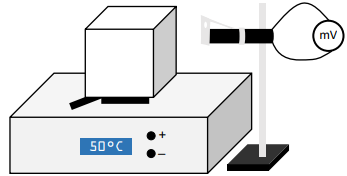
\includegraphics[scale=0.5]{cube}
	\caption{Schemat układu do pomiarów z kostką Lesliego (źródło: \cite{skrypt}). Po lewej stronie widzimy kostkę, w centrum detektor promieniowania, a po prawej miernik napięcia.}
	\label{fig:cube_diagram}
\end{figure}

Kostka ma cztery powierzchnie: czarną, białą, metalową matową oraz metalową błyszczącą. Każdą z nich nagrzewamy do wybranej temperatury, po czym mierzymy napięcie w detektorze. Kluczowym etapem jest zasłanianie detektora podczas nagrzewania kostki, by uniknąć przegrzewania samego czujnika.
Przy najwyższej temperaturze kostki, sprawdzamy co się stanie gdy między detektor a ścianę czarną włożymy szklany ekran.

\subsection{Lampa Stefana–Boltzmanna}
W drugiej części weryfikujemy prawo Stefana–Boltzmanna, używając żarówki i detektora, ustawionych na szynie z zaznaczonymi odległościami (rys.~\ref{fig:lamp_diagram}). 

\begin{figure}[H]
	\centering
	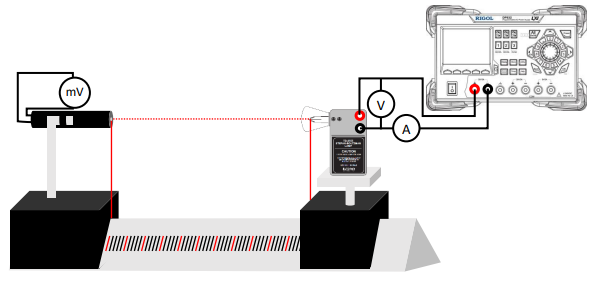
\includegraphics[scale=0.5]{lamp}
	\caption{Schemat układu z żarówką i detektorem (źródło: \cite{skrypt}). Po lewej stronie, na szynie, znajduje się detektor promieniowania z podłączonym miernikiem napięcia, w centrum widzimy żarówkę z obwodem podłączonym do generatora napięcia umieszczonego po prawej.}
	\label{fig:lamp_diagram}
\end{figure}

Najpierw mierzymy zależność promieniowania od temperatury żarówki (przez zmianę napięcia i prądu w obwodzie). Temperaturę włókna obliczamy ze wzorów \cite{skrypt}:
\begin{equation}
	T = \frac{R - R_{\mathrm{ref}}}{\alpha\,R_{\mathrm{ref}}} + T_{\mathrm{ref}},
	\label{eq:temp_bulb}
\end{equation}
gdzie $T_{\mathrm{ref}}=300\,\mathrm{K}$, $R_{\mathrm{ref}}=0{,}277\,\Omega$, zaś $\alpha$ zależy od $R$ w sposób określony eksperymentalnie \cite{skrypt}. 
\[
    \alpha = 0{,}00407\cdot \left(\frac{R}{R_{\mathrm{ref}}}\right)^{0{,}11778}
\]
Po ustaleniu najwyższej temperatury żarówki sprawdzamy, co się stanie po wstawieniu szklanego ekranu między żarówkę a detektor. 
W kolejnym etapie badamy zależność natężenia promieniowania od odległości, utrzymując temperaturę żarówki (a więc i jej moc promieniowania) na stałym poziomie.

\section{Wyniki Pomiarów}
Wszystkie pomiary wykonaliśmy w pomieszczeniu o stałej temperaturze $T_0 = 22\,^\circ\mathrm{C}$. W analizie błędów oznaczamy:
\[
\bar{x} \;(\text{średnia}),\quad s_x \;(\text{błąd statystyczny}),\quad \delta x \;(\text{błąd pojedynczego pomiaru}),\quad u(x)\;(\text{błąd całkowity}).
\]
Łączny błąd w przypadku wielu punktów (suma błędu statystycznego i pomiarowego) definiujemy jako:
\begin{equation}
	u(x) = \sqrt{s_x^2 + \Bigl(\frac{\delta x}{\sqrt{3}}\Bigr)^2},
	\label{eq:combined_error}
\end{equation}
a dla pojedynczego pomiaru przyjmujemy $u(x) = \delta x$. Korzystamy też z klasycznej propagacji niepewności:
\begin{equation}
	\delta f(x) = \sqrt{\sum_{i}\bigl(\frac{\partial f}{\partial x_i}\,\delta x_i\bigr)^2}.
	\label{eq:error_propagation}
\end{equation}
Do testowania jakości dopasowania używamy testu $\chi^2$:
\begin{equation}
	\chi^2 = \sum_{i} \frac{\bigl[y_i - f(x_i)\bigr]^2}{\sigma_{y_i}^2 + \Bigl(\frac{df}{dx_i}\,\sigma_{x_i}\Bigr)^2}.
	\label{eq:chi2}
\end{equation}

\subsection{Kostka Lesliego}
Tabela \ref{tab:cube_measurements} zawiera dane z badania kostki Lesliego: napięcie detektora dla stron czarnej ($U_b$), białej ($U_w$), metalowej błyszczącej ($U_{ms}$), metalowej matowej ($U_{mm}$) oraz sygnał tła $U_s$ (gdy kostka jest zasłonięta).

\begin{table}[H]
	\centering
	\begin{tabular}{c|c|cccc|c}
		\toprule
		Nr & $T\,[^\circ \mathrm{C}]$ & $U_b\,[\mathrm{mV}]$ & $U_w\,[\mathrm{mV}]$ & $U_{ms}\,[\mathrm{mV}]$ & $U_{mm}\,[\mathrm{mV}]$ & $U_s\,[\mathrm{mV}]$ \\
		\midrule
		1  & 50 & 2{,}05 & 2{,}05 & 0{,}17 & 0{,}53 & 0{,}15 \\
		2  & 55 & 2{,}56 & 2{,}56 & 0{,}18 & 0{,}63 & 0{,}15 \\
		3  & 60 & 2{,}94 & 2{,}93 & 0{,}23 & 0{,}71 & 0{,}15 \\
		4  & 65 & 3{,}45 & 3{,}41 & 0{,}25 & 0{,}80 & 0{,}17 \\
		5  & 70 & 3{,}89 & 3{,}89 & 0{,}26 & 0{,}95 & 0{,}21 \\
		6  & 75 & 4{,}43 & 4{,}40 & 0{,}29 & 1{,}04 & 0{,}19 \\
		7  & 80 & 4{,}97 & 4{,}94 & 0{,}32 & 1{,}16 & 0{,}17 \\
		8  & 85 & 5{,}43 & 5{,}41 & 0{,}34 & 1{,}28 & 0{,}14 \\
		9  & 90 & 5{,}95 & 5{,}85 & 0{,}38 & 1{,}39 & 0{,}14 \\
		10 & 95 & 6{,}52 & 6{,}48 & 0{,}42 & 1{,}53 & 0{,}17 \\
		11 & 100 & 7{,}12 & 7{,}06 & 0{,}45 & 1{,}71 & 0{,}19 \\
		12 & 105 & 7{,}66 & 7{,}63 & 0{,}50 & 1{,}85 & 0{,}21 \\
		13 & 110 & 8{,}34 & 8{,}32 & 0{,}54 & 2{,}06 & 0{,}24 \\
		14 & 115 & 8{,}87 & 8{,}85 & 0{,}58 & 2{,}15 & 0{,}26 \\
		15 & 120 & 9{,}52 & 9{,}52 & 0{,}63 & 2{,}34 & 0{,}25 \\
		\bottomrule
	\end{tabular}
    \caption{Pomiary napięć dla różnych ścian kostki Lesliego czarna $U_b$, biała $U_2$, metalowa błyszcząca $U_{ms}$, metalowa matowa $U_{mm}$i napięcia wywoływanego przez pomieszczenie ($U_s$) w zależności od temperatury $T$.}
	\label{tab:cube_measurements}
\end{table}

Widać, że ściany czarna i biała dają porównywalne sygnały, podczas gdy metalowa błyszcząca jest niemal na poziomie tła ($U_s$), a metalowa matowa ma wartości pośrednie. Następnie w obliczeniach odejmujemy średni sygnał tła $\bar{U_s}$, aby otrzymać $U' = U - \bar{U_s}$. Zakładamy też niepewności pomiarowe: $\delta T \approx 1\,^\circ\mathrm{C}$ oraz wyznaczamy $\delta U$ z instrukcji multimetru \cite{radiation_multimeter}.

Aby sprawdzić zgodność z prawem Stefana–Boltzmanna, wykreślamy $U'$ w zależności od $T^4$ i dopasowujemy linię (rys.~\ref{fig:cube_temp}).

\begin{figure}[H]
	\centering
	\begin{subfigure}{0.45\textwidth}
		\centering
		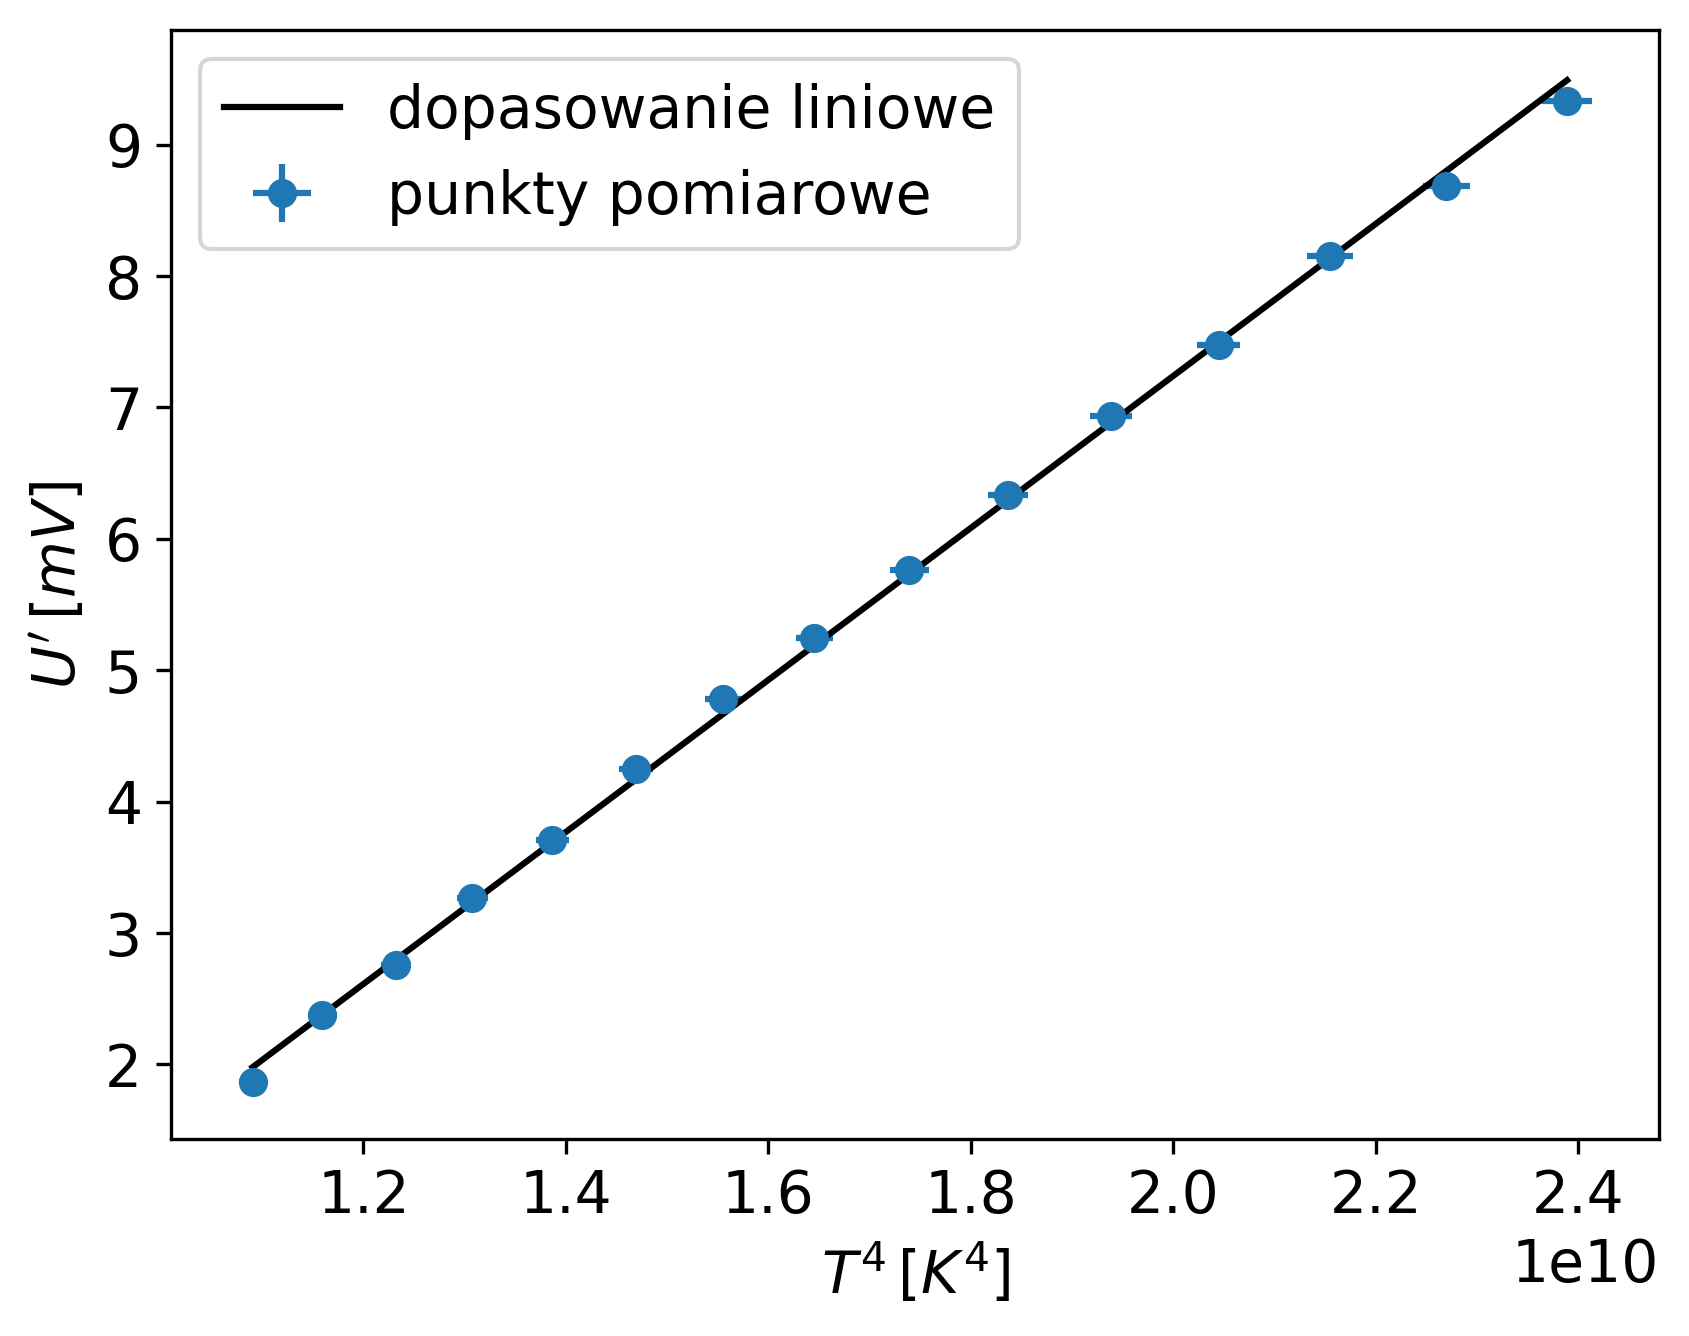
\includegraphics[width=\linewidth]{cube_black}
		\caption{Ściana czarna}
		\label{fig:cube_black}
	\end{subfigure}
	\hfill
	\begin{subfigure}{0.45\textwidth}
		\centering
		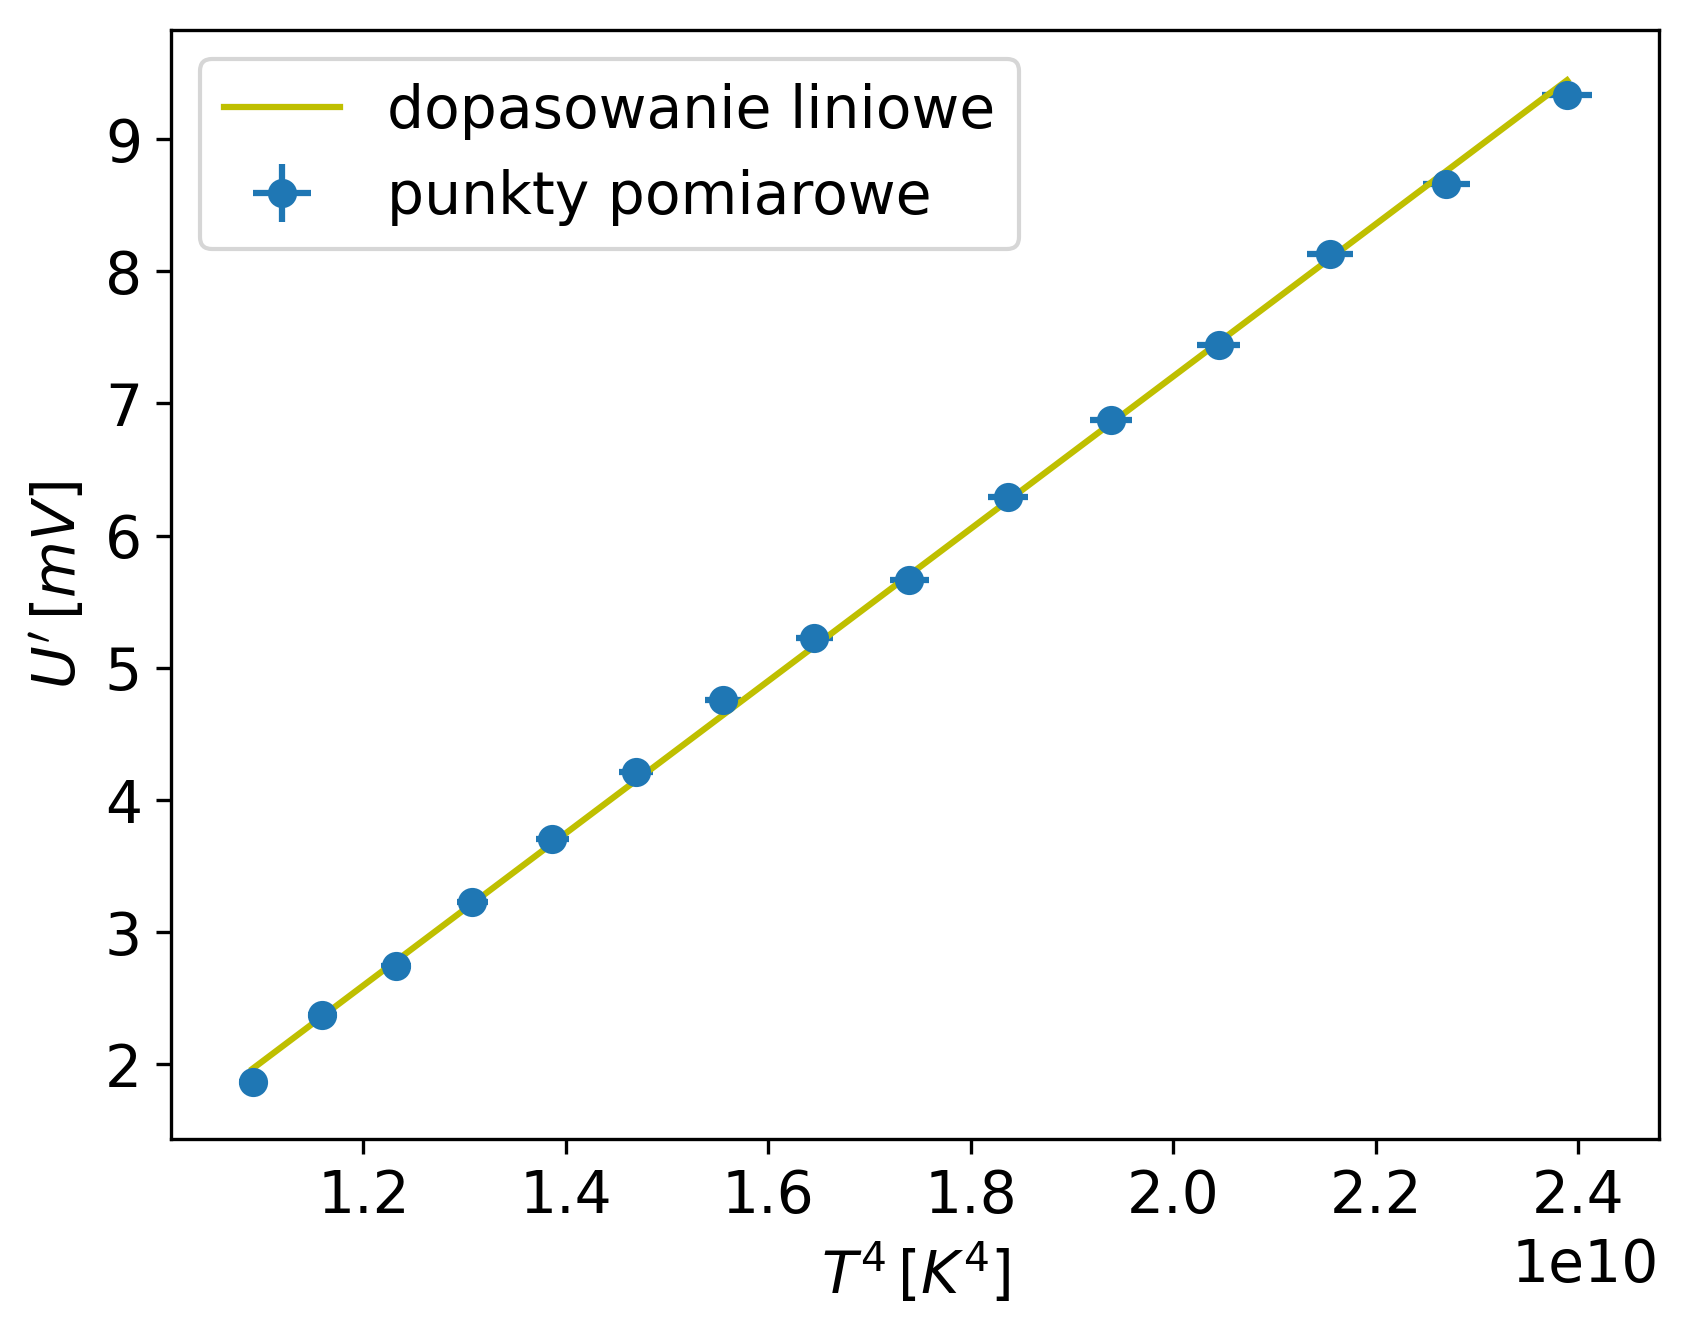
\includegraphics[width=\linewidth]{cube_white}
		\caption{Ściana biała}
		\label{fig:cube_white}
	\end{subfigure}

	\vspace{1em}

	\begin{subfigure}{0.45\textwidth}
		\centering
		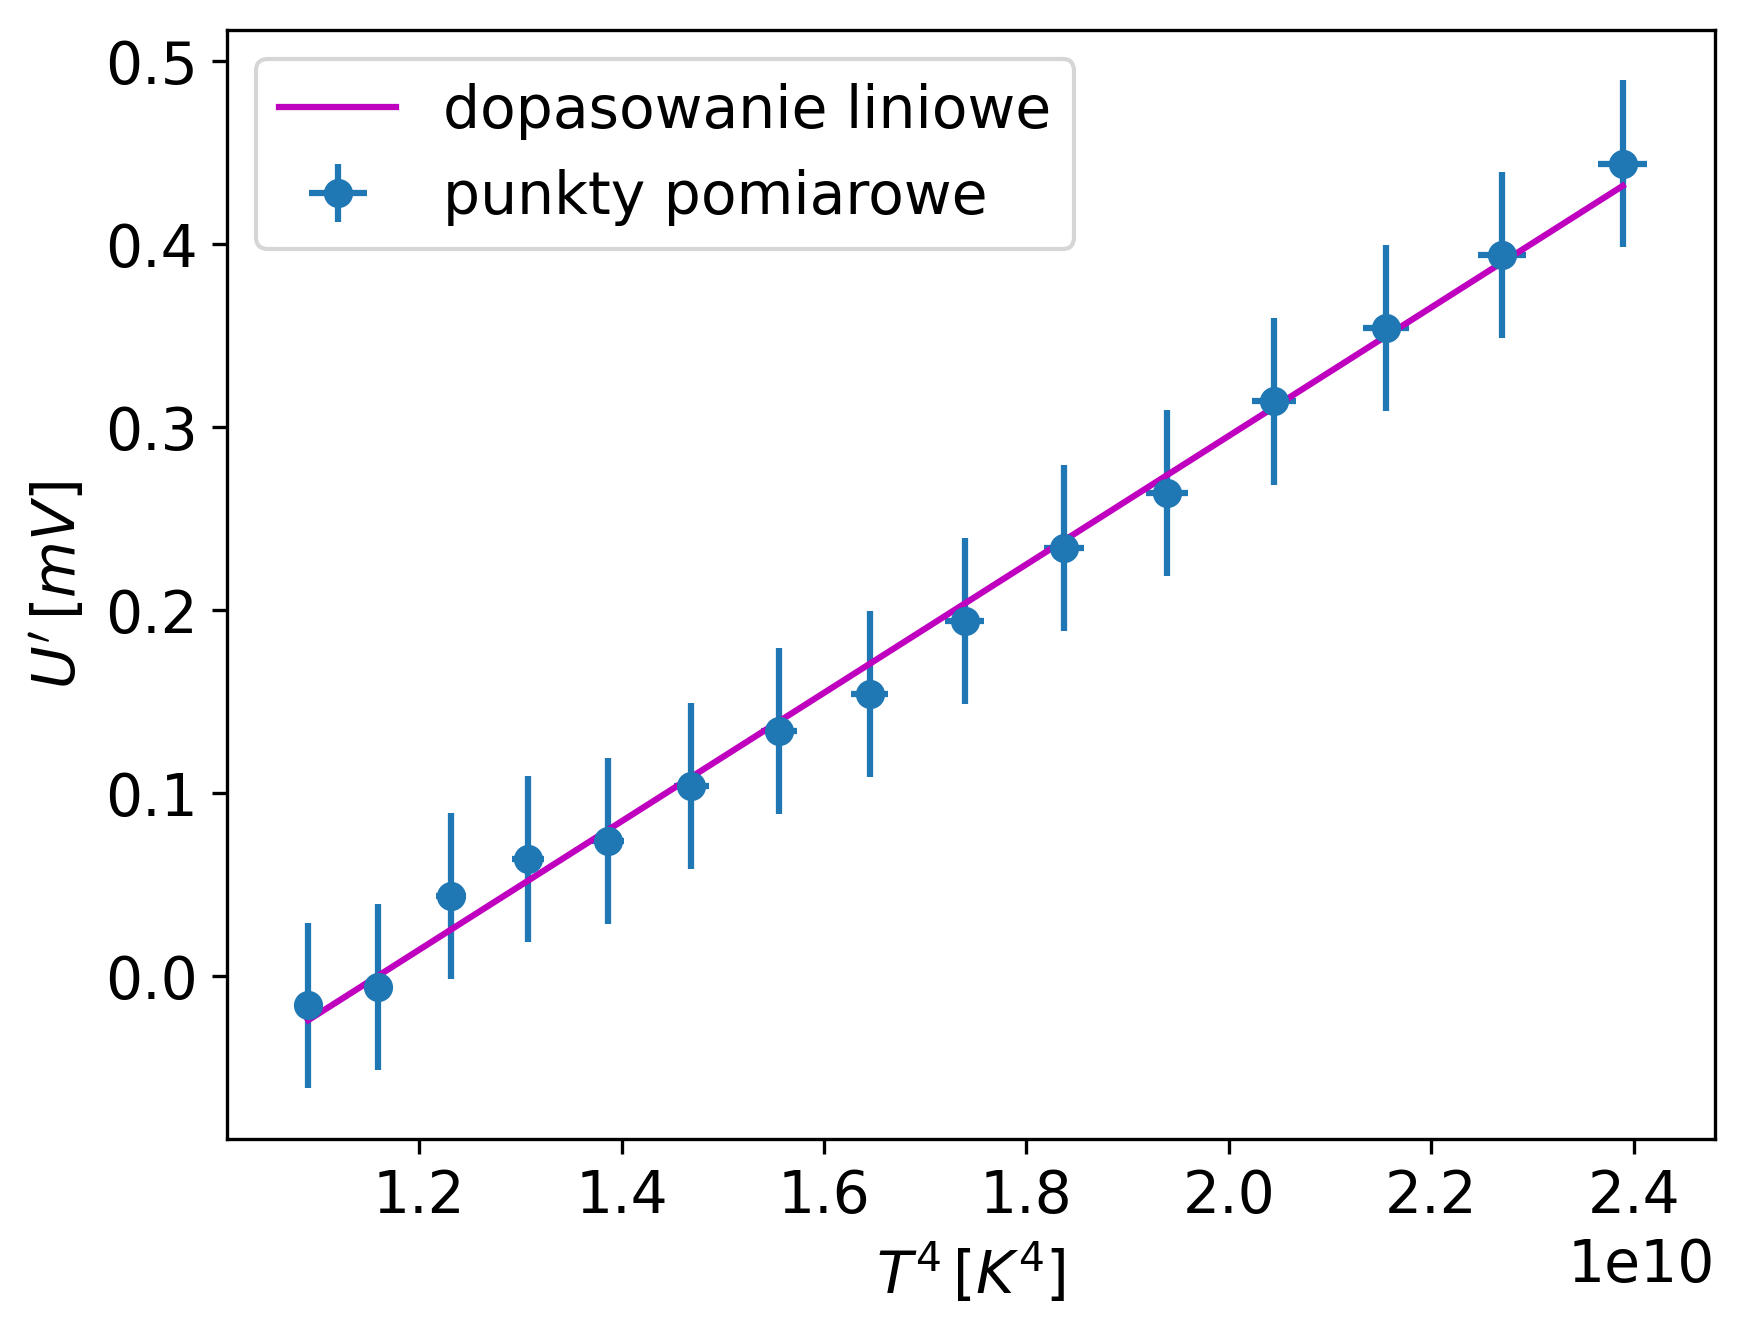
\includegraphics[width=\linewidth]{cube_shining}
		\caption{Metalowa błyszcząca}
		\label{fig:cube_shining}
	\end{subfigure}
	\hfill
	\begin{subfigure}{0.45\textwidth}
		\centering
		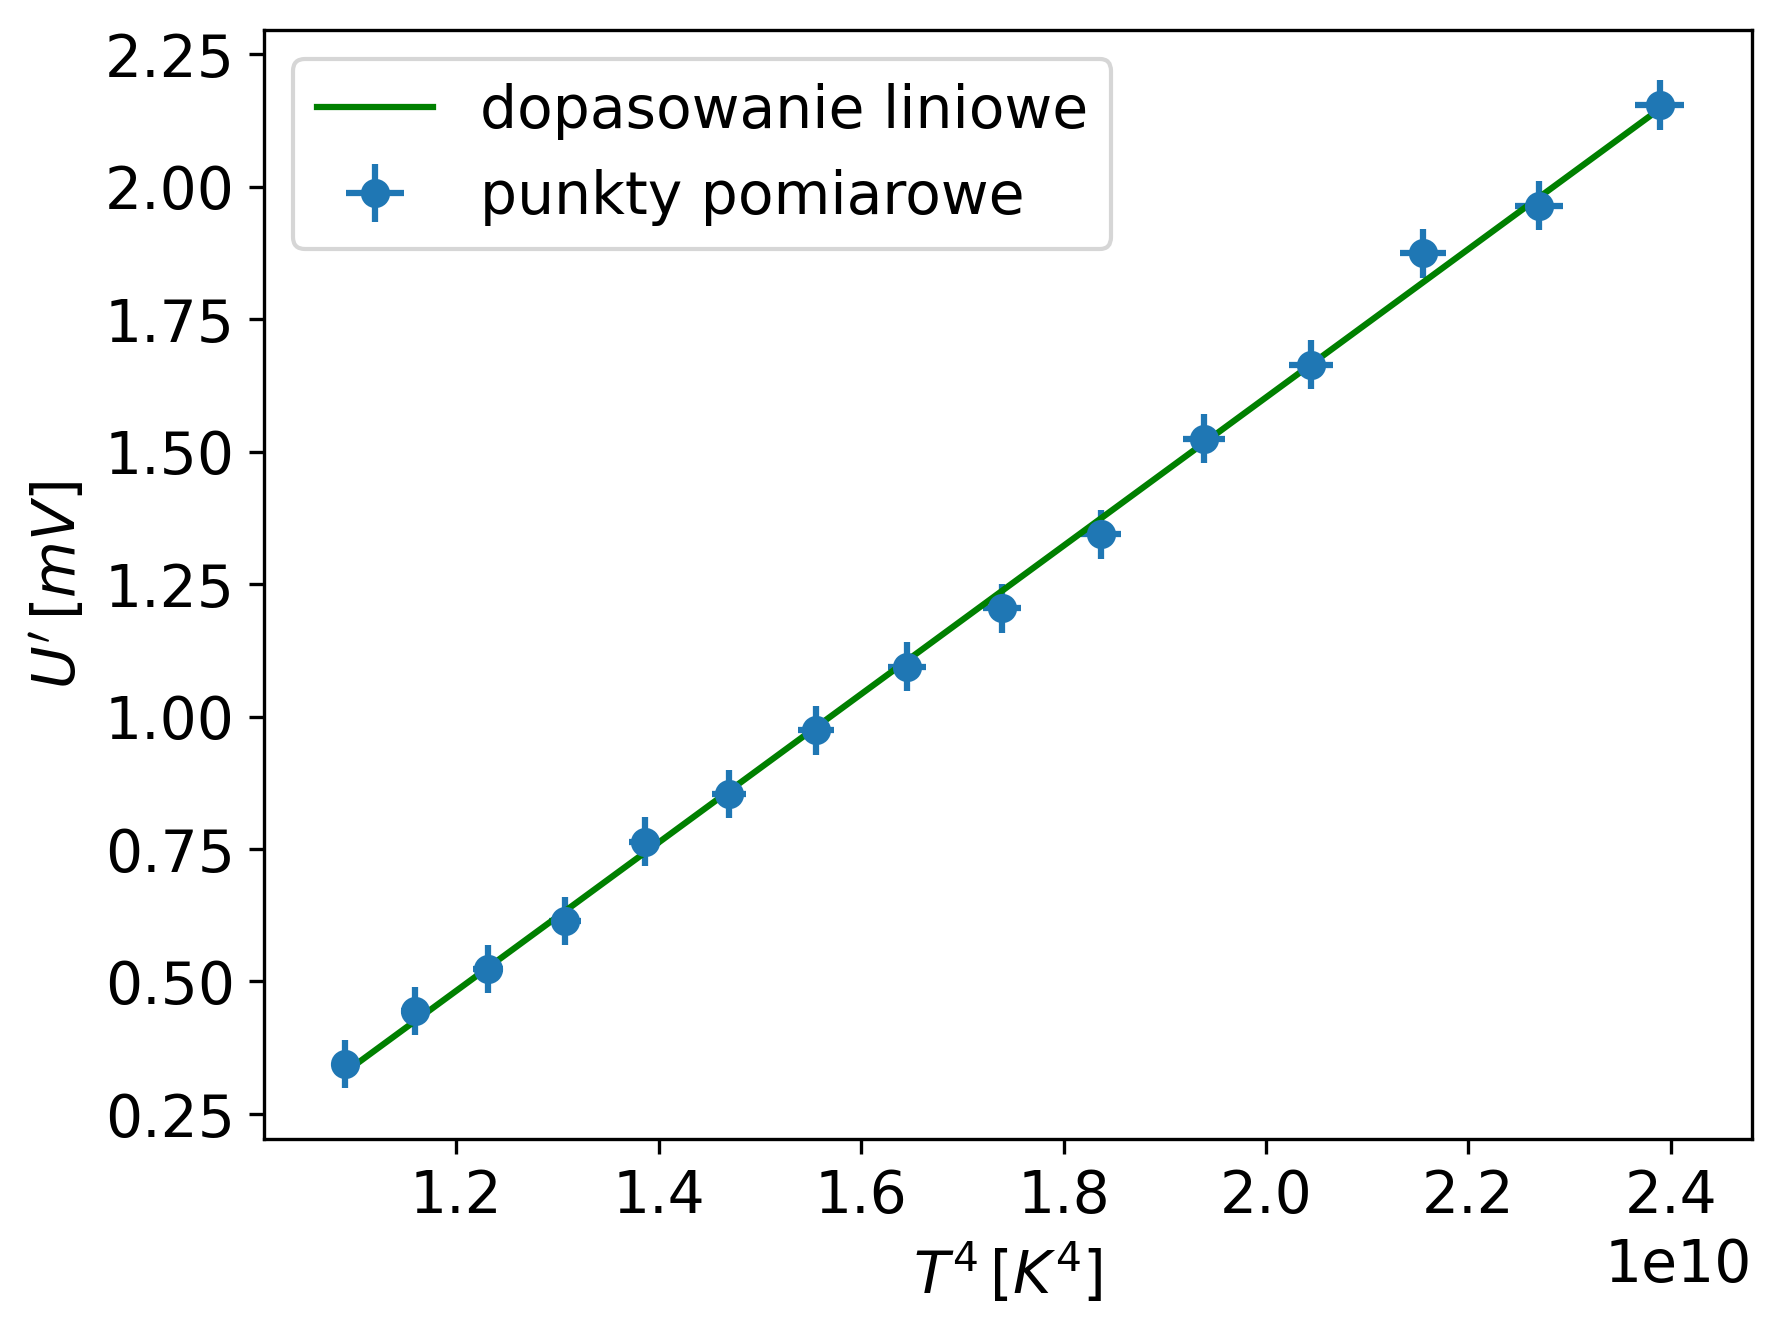
\includegraphics[width=\linewidth]{cube_dull}
		\caption{Metalowa matowa}
		\label{fig:cube_dull}
	\end{subfigure}
	\caption{Zależność napięcia $U'$ (zredukowanego o tło) od $T^4$ dla różnych ścian kostki Lesliego.}
	\label{fig:cube_temp}
\end{figure}

Współczynniki kierunkowe $a$ z dopasowanych prostych podsumowano w tab.~\ref{tab:cube_line}.

\begin{table}[H]
	\centering
	\begin{tabular}{c|cc}
		\toprule
		Materiał ściany & $a\,[pV\,K^{-4}]$ & $u(a)\,[pV\,K^{-4}]$ \\
		\midrule
		Czarna           & 0{,}578  & 0{,}006 \\
		Biała            & 0{,}576  & 0{,}005 \\
		Metal błyszcząca & 0{,}0351 & 0{,}0007 \\
		Metal matowa     & 0{,}1400 & 0{,}0015 \\
		\bottomrule
	\end{tabular}
	\caption{Współczynniki kierunkowe dopasowania w zależności $U'(T^4)$ dla kostki Lesliego.}
	\label{tab:cube_line}
\end{table}

Załóżmy, że ściana czarna ma emisyjność $\epsilon_b=0{,}95$ oraz że emisyjność dla każdej ze ścian jest stała i nie zależy od długości emitowanych fal (co za tym idzie temperatury). Wówczas, porównując współczynniki kierunkowe (podczas pomiarów układ był stacjonarny, jedynie kostka obracała się w miejscu), obliczamy emisyjności innych ścian za pomocą:
\begin{equation}
	\epsilon_o = \epsilon_b\,\frac{a_o}{a_b}, 
	\quad
	u(\epsilon_o) = \epsilon_o\,\sqrt{\Bigl(\frac{u(a_o)}{a_o}\Bigr)^2 + \Bigl(\frac{u(a_b)}{a_b}\Bigr)^2}.
	\label{eq:epsilon_ratio}
\end{equation}
Wyniki przedstawia tab.~\ref{tab:materials_emisity}.

\begin{table}[H]
	\centering
	\begin{tabular}{c|cc}
		\toprule
		Materiał ściany & $\epsilon$ & $u(\epsilon)$ \\
		\midrule
		Biała            & 0{,}946    & 0{,}011 \\
		Metal błyszcząca & 0{,}0576   & 0{,}0012 \\
		Metal matowa     & 0{,}230    & 0{,}003 \\
		\bottomrule
	\end{tabular}
	\caption{Wyznaczone emisyjności dla ścian kostki przy założeniu, że strona czarna ma $\epsilon=0{,}95$.}
	\label{tab:materials_emisity}
\end{table}

\subsection{Żarówka Boltzmanna}
\paragraph{Pomiar zależności od temperatury.}
Dla żarówki ustawionej w odległości $r=5\,\mathrm{cm}$ od detektora, zmienialiśmy napięcie $U_l$ i prąd $I_l$ na żarówce przy pomocy multimetru. W tab.~\ref{tab:temp_measurements} zestawiono odczyty z multimetru $U_d$ i napięcie tła $U_s$ (przy zasłoniętym detektorze) dla detektora, a także temperaturę obliczoną ze wzorów \eqref{eq:temp_bulb}.

\begin{table}[H]
	\centering
	\begin{tabular}{c|cc|c|c|cc}
		\toprule
		Nr & $U_l$ [V] & $I_l$ [A] & $U_d$ [mV] & $U_s$ [mV] & $T$ [K] & $\delta T$ [K]\\
		\midrule
		1  & 0{,}828   & 0{,}919 & 0{,}15  & 0{,}05 & 781{,}69  & 18{,}81 \\
		2  & 1{,}775   & 1{,}191 & 1{,}13  & 0{,}05 & 1182{,}75 & 27{,}41 \\
		3  & 2{,}725   & 1{,}432 & 2{,}89  & 0{,}05 & 1449{,}35 & 32{,}87 \\
		4  & 3{,}681   & 1{,}648 & 5{,}68  & 0{,}07 & 1657{,}25 & 37{,}06 \\
		5  & 4{,}64    & 1{,}847 & 9{,}12  & 0{,}08 & 1829{,}17 & 44{,}02 \\
		6  & 5{,}60    & 2{,}033 & 12{,}31 & 0{,}06 & 1976{,}70 & 46{,}42 \\
		7  & 6{,}57    & 2{,}207 & 16{,}15 & 0{,}09 & 2110{,}54 & 48{,}71 \\
		8  & 7{,}53    & 2{,}370 & 20{,}25 & 0{,}08 & 2230{,}01 & 50{,}81 \\
		9  & 8{,}50    & 2{,}524 & 25{,}13 & 0{,}10 & 2342{,}70 & 52{,}84 \\
		10 & 9{,}47    & 2{,}671 & 30{,}24 & 0{,}11 & 2447{,}17 & 54{,}76 \\
		\bottomrule
	\end{tabular}
	\caption{Pomiary napięcia detektora $U_d$ i tła $U_s$, napięcia i prądu żarówki ($U_l$, $I_l$) oraz wyliczonej temperatury włókna $T$.}
	\label{tab:temp_measurements}
\end{table}

Po odjęciu tła średniej z tła $\bar{U_s}$ otrzymujemy $U' = U_d - \bar{U_s}$ i dopasowujemy zależność $U' = a_{l_t}\,T^4 + b_{l_t}$ (rys.~\ref{fig:boltzman_temp}).

\begin{figure}[H]
	\centering
	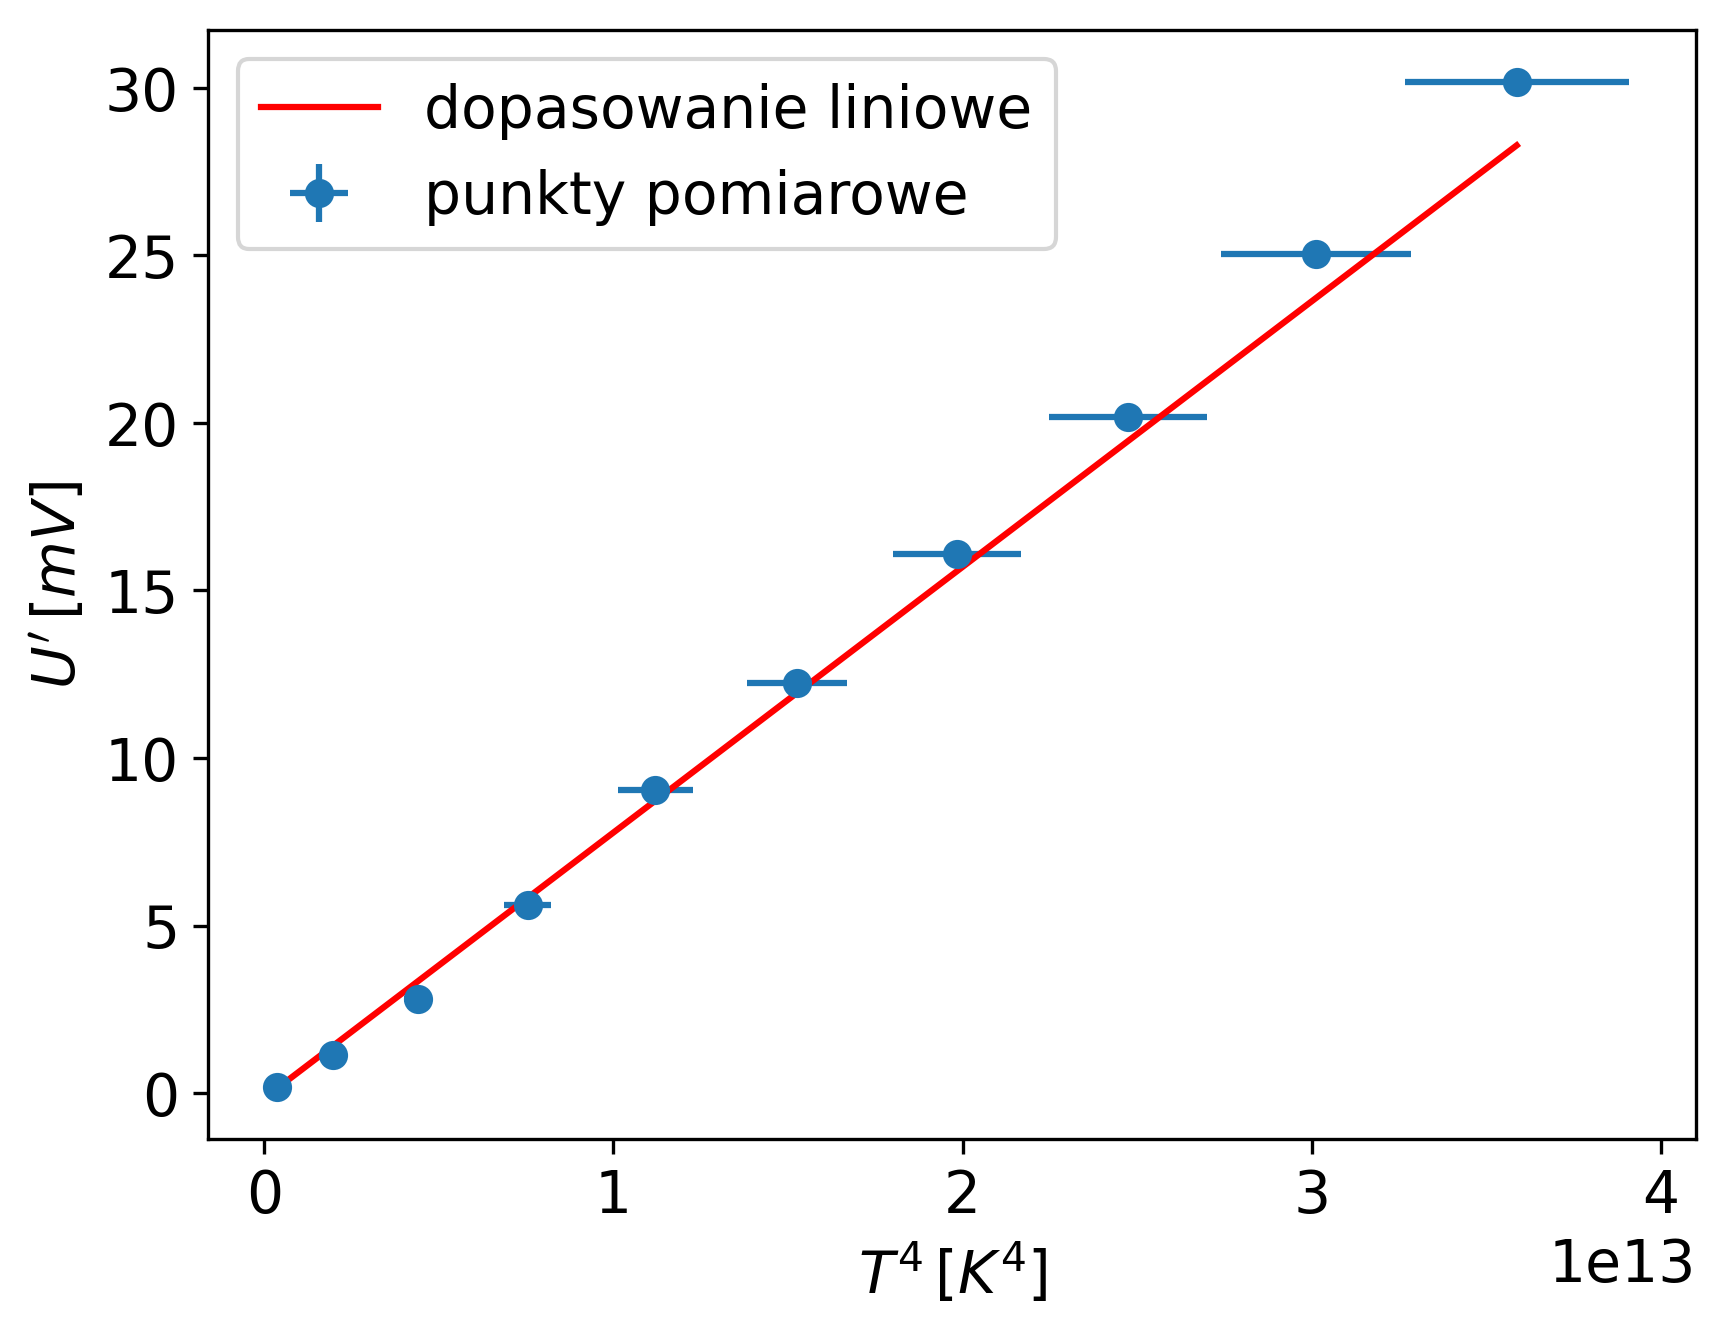
\includegraphics[scale=0.6]{boltzman_temp}
	\caption{Zależność $U'$ od $T^4$ dla żarówki (zmienna temperatura, stała odległość).}
	\label{fig:boltzman_temp}
\end{figure}

Wyznaczone parametry:
\[
	a_{l_t} = (0{,}79 \pm 0{,}03) \times 10^{-15}\,[VK^{-4}], 
	\quad 
	b_{l_t} = (-0{,}15 \pm 0{,}05) \,[mV].
\]
Test $\chi^2$ \eqref{eq:chi2} daje $\chi^2=8{,}36$ przy $8$ stopniach swobody, co wskazuje na dobrą zgodność z modelem Stefana–Boltzmanna.

\paragraph{Pomiar zależności od odległości.}
Przy stałych parametrach żarówki ($U_l=9{,}47\,\mathrm{V}$, $I_l=2{,}670\,\mathrm{A}$, odległość $r$ odczytywana na szynie) uzyskane wyniki zamieszczono w tab.~\ref{tab:distance_measurements}.

\begin{table}[H]
	\centering
	\begin{tabular}{c|c|c|c}
		\toprule
		Nr & $d\,[\mathrm{cm}]$ & $U_d\,[\mathrm{mV}]$ & $U_s\,[\mathrm{mV}]$ \\
		\midrule
		1  & 149 & 30{,}58 & 0{,}12 \\
		2  & 144 & 9{,}29  & 0{,}10 \\
		3  & 139 & 4{,}11  & 0{,}11 \\
		4  & 134 & 2{,}36  & 0{,}11 \\
		5  & 129 & 1{,}52  & 0{,}11 \\
		6  & 124 & 1{,}08  & 0{,}08 \\
		7  & 119 & 0{,}82  & 0{,}06 \\
		8  & 114 & 0{,}64  & 0{,}05 \\
		9  & 109 & 0{,}52  & 0{,}05 \\
		\bottomrule
	\end{tabular}
	\caption{Pomiary napięcia $U_d$ przy różnych odległościach $d$. $U_s$ to napięcie tła.}
	\label{tab:distance_measurements}
\end{table}

Zakładamy, że odległość rzeczywista wynosi $r = |d - d_0|$, gdzie $d_0=154\,\mathrm{cm}$, a błąd z jakim mierzyliśmy odległość wynosi połowę podziałki szyny $u(d) = 0{,}05 \, \mathrm{cm}$. Po odjęciu tła otrzymujemy $U'$, a następnie weryfikujemy zależność $\log(U')$ od $\log(r)$ (rys.~\ref{fig:boltzman_distance}).

\begin{figure}[H]
	\centering
	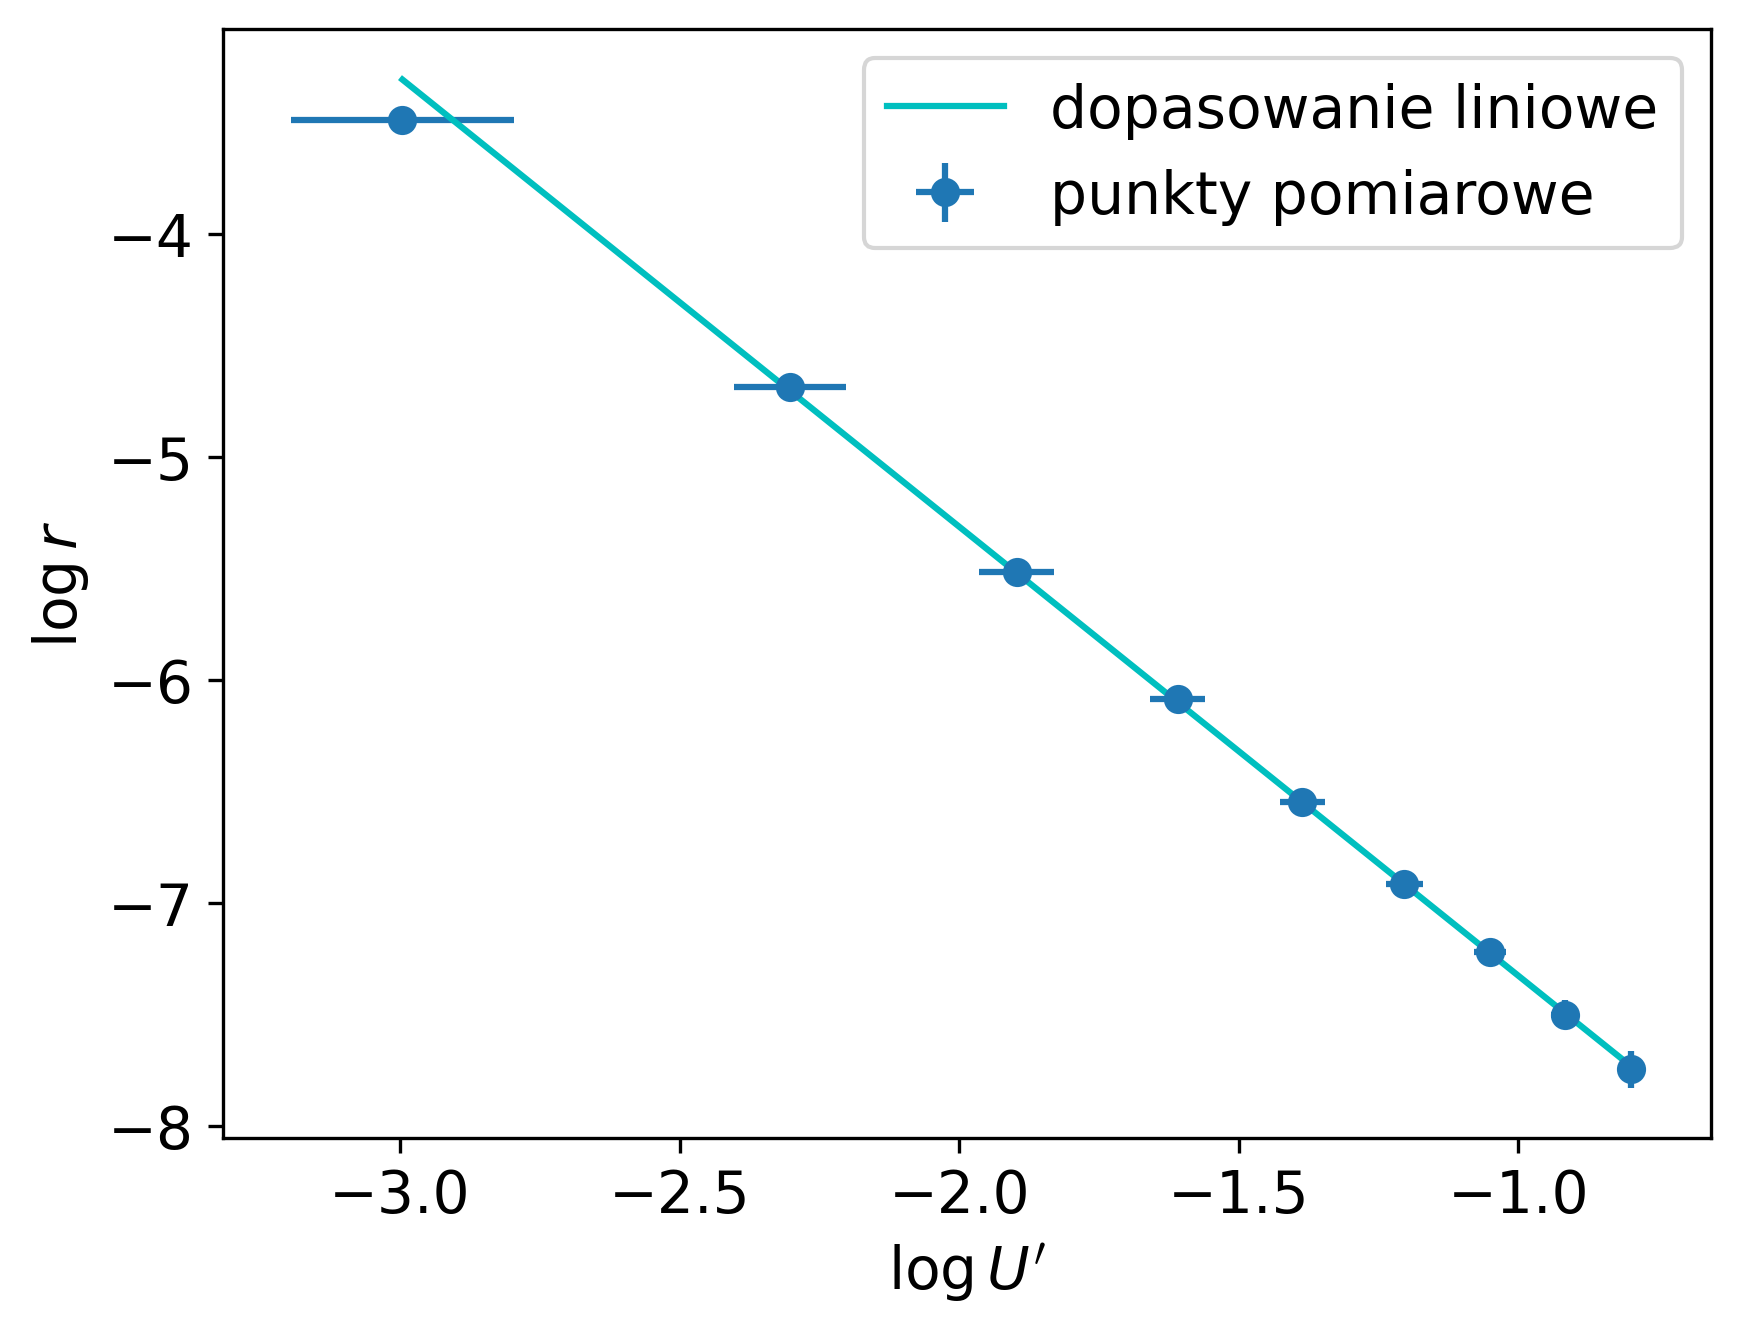
\includegraphics[scale=0.6]{boltzman_distance}
	\caption{Zależność $\log(U')$ od $\log(r)$ dla żarówki utrzymywanej w stałej temperaturze.}
	\label{fig:boltzman_distance}
\end{figure}

Uzyskane parametry dopasowania:
\[
	a_{l_d}=-2{,}013 \pm 0{,}017, 
	\quad 
	b_{l_d}=-9{,}34 \pm 0{,}03.
\]
Test $\chi^2=0{,}97$ przy $7$ stopniach swobody potwierdza, że $U'\propto r^{-2}$, czyli zgodnie z równaniem \eqref{eq:power_flux}.

\subsection{Transmisyjność Szkła}
Na koniec porównaliśmy wskazania detektora z i bez szklanego ekranu. Dla kostki Lesliego (nagrzanej do $150^\circ\mathrm{C}$) oraz żarówki ($>2000^\circ\mathrm{C}$) zebrane dane przedstawiono w tab.~\ref{tab:cube_glass} i \ref{tab:bulb_glass}.

\begin{table}[H]
	\centering
	\begin{tabular}{cc}
		\toprule
		Pomiar      & $U_d\,[\mathrm{mV}]$ \\
		\midrule
		Bez szkła   & 9{,}53 \\
		Z ekranem   & 0{,}19 \\
		\bottomrule
	\end{tabular}
	\caption{Kostka Lesliego (T=150$^\circ$C) z ekranem szklanym i bez.}
	\label{tab:cube_glass}
\end{table}

\begin{table}[H]
	\centering
	\begin{tabular}{cc}
		\toprule
		Pomiar      & $U_d\,[\mathrm{mV}]$ \\
		\midrule
		Bez szkła   & 30{,}24 \\
		Z ekranem   & 22{,}10 \\
		\bottomrule
	\end{tabular}
	\caption{Żarówka ($T\!>\!2000^\circ\mathrm{C}$) z ekranem szklanym i bez.}
	\label{tab:bulb_glass}
\end{table}

W przypadku kostki (emitującej głównie promieniowanie w podczerwieni) szkło niemal całkowicie blokuje docierający strumień (wskazania maleją do wartości tła). Natomiast dla żarówki, której emisja zawiera znaczną składową widzialną (wysoka temperatura), sygnał spada mniej gwałtownie (ok. 73\% wartości pierwotnej). Zgodne jest to z wiedzą, że powrzechne szkło jest w dużym stopniu nieprzezroczyste w podczerwieni, a dobrze przepuszcza światło widzialne (rys.~\ref{fig:black_body}).

\begin{figure}[H]
	\centering
	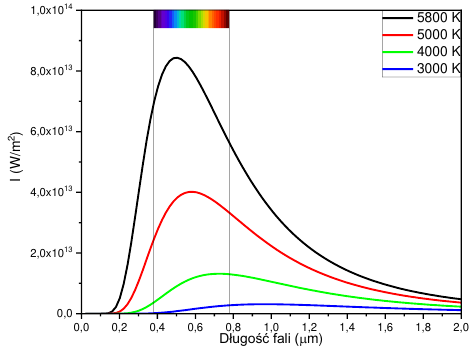
\includegraphics[scale=0.65]{black_body}
	\caption{Zależność widmowa ciała doskonale czarnego (źródło: \cite{skrypt}).}
	\label{fig:black_body}
\end{figure}

\section{Podsumowanie}
W przedstawionym doświadczeniu rozpoczęliśmy od analizy kostki Lesliego. Zmierzyliśmy zależność napięcia w detektorze od temperatury kostki (tab.~\ref{tab:cube_measurements}), przyjmując, że wskazanie detektora jest liniowe względem natężenia promieniowania. Otrzymaliśmy proste dopasowania do wykresu $U'\bigl(T^4\bigr)$ (rys.~\ref{fig:cube_temp}). Przy założeniu $\epsilon_{\text{black}}=0{,}95$ dla ściany czarnej wyznaczyliśmy emisyjność pozostałych ścian (tab.~\ref{tab:materials_emisity}): 
\[
\epsilon_{\text{white}} = 0{,}946 \pm 0{,}011,\quad
\epsilon_{\text{metal~mat.}} = 0{,}230 \pm 0{,}003,\quad
\epsilon_{\text{metal~bł.}} = 0{,}0576 \pm 0{,}0012.
\]

Następnie zbadaliśmy żarówkę o regulowanej temperaturze (tab.~\ref{tab:temp_measurements}), dopasowując zależność $U' = a_{l_t}\,T^4 + b_{l_t}$ (rys.~\ref{fig:boltzman_temp}), co dało 
\[
    a_{l_t} = (0{,}79 \pm 0{,}03) \times 10^{-15}\,[VK^{-4}] \quad \text{oraz} \quad b_{l_t} = (-0{,}15 \pm 0{,}05) \, [mV]
\]
zweryfikowane testem $\chi^2$ (uzyskano $\chi^2=8{,}36$ przy 8 stopniach swobody). Przy stałej temperaturze żarówki (tab.~\ref{tab:distance_measurements}) zmienialiśmy odległość do detektora, otrzymując wyniki zgodne z zależnością $U'\propto 1/r^2$ (rys.~\ref{fig:boltzman_distance}), z parametrem nachylenia $a_{l_d}=-2{,}013 \pm 0{,}017$ (test $\chi^2=0{,}97$ przy $7$ stopniach swobody). 

Ostatecznie z pomiarów z ekranem szklanym (tab.~\ref{tab:cube_glass}, \ref{tab:bulb_glass}) wnioskujemy, że szkło niemal całkowicie blokuje promieniowanie podczerwone (silny spadek sygnału przy kostce ~150$^\circ$C), ale przepuszcza znaczną część promieniowania widzialnego (mniejszy spadek dla żarówki >2000$^\circ$C).

Porównując uzyskane wyniki z danymi producenta kostki Lesliego \cite{cube}, widzimy pewne różnice w wartościach emisyjności (szczególnie ścian metalowych). Różnice te mogą wynikać z nagrzewania się detektora (zwłaszcza przy dłuższym pomiarze ścian czarnych i białych), a także z niedokładności ustabilizowania się napięcia i ewentualnego ogrzewania zasłony. 
Analiza przepuszczalności szkła \cite{glass} pokazuje, że przy typowych rodzajach szkła transmisja silnie spada w obszarze podczerwonym, co jest zgodne z naszymi obserwacjami.
W przypadku pomiarów z żarówką test $\chi^2$ potwierdził powrzechnie przyjmowane prawa dyktujące zachowanie emitowanego promieniowania.

\newpage
\begin{thebibliography}{5}

	\bibitem{skrypt}
	\emph{Badanie Promieniowania Termicznego}, Uniwersytet Warszawski, Aneta Drabińska.

	\bibitem{radiation_multimeter}
	\url{brymen.eu/wp-content/uploads/biall/102091/102091.KARTA_EN..2015-07-08.1.pdf}, miernik uniwersalny BRYMEN BM827s.

	\bibitem{bulb_multimeter}
	\url{https://static.eleshop.nl/mage/media/downloads/bm805_datasheet.pdf}, miernik uniwersalny BRYMEN BM805s.

    \bibitem{cube}
    \url{https://www.3bscientific.com/product-manual/UE2020205-230_EN2.pdf}, kostka Lesliego.

    \bibitem{glass}
    \url{https://wp.optics.arizona.edu/optomech/wp-content/uploads/sites/53/2016/10/tie-35_transmittance_us.pdf}, Schott (analizy transmisji szkła).

\end{thebibliography}

\end{document}
